\documentclass{article}
\usepackage{tikz}
\usetikzlibrary{arrows.meta,positioning,calc,shapes.geometric}
\pagestyle{empty}
\begin{document}
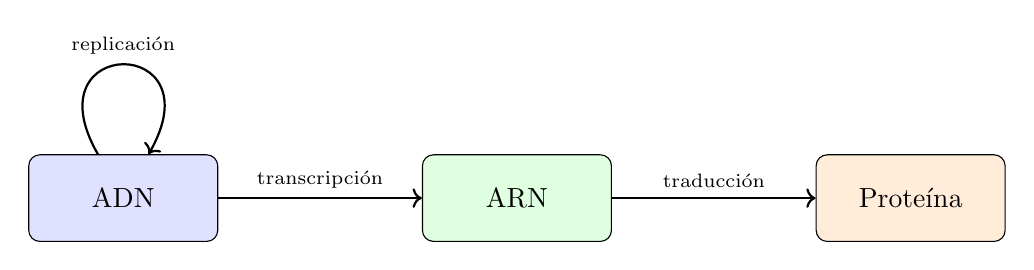
\begin{tikzpicture}

\node[draw, rounded corners, fill=blue!12, minimum width=2.4cm, minimum height=1.1cm] (a) at (0,0) {ADN};
\node[draw, rounded corners, fill=green!12, minimum width=2.4cm, minimum height=1.1cm] (r) at (5,0) {ARN};
\node[draw, rounded corners, fill=orange!15, minimum width=2.4cm, minimum height=1.1cm] (p) at (10,0) {Proteína};
\draw[->, thick] (a) -- node[above, font=\scriptsize] {transcripción} (r);
\draw[->, thick] (r) -- node[above, font=\scriptsize] {traducción} (p);
\draw[->, thick] (a) to[out=120, in=60, looseness=7] node[above, font=\scriptsize] {replicación} (a);

\end{tikzpicture}
\end{document}
